% =====================================================================================================
% Drop-in text for the H2 and mechanism parts of the report, in the report's notation.
% Each block says which part of medsa_robustness_report_preview.pdf it replaces.
% ?? = value not in this hand-off; run code/report_numbers.py on stats.json / feature_stats.csv to fill it.
% \cite{gu2022} is a placeholder key for reference [11] (Gu, Tresp and Qin, ECCV 2022): use the report's key.
% Requires: \usepackage{graphicx}. Figure paths assume the figures/ folder sits next to the .tex file.
% =====================================================================================================


% -----------------------------------------------------------------------------------------------------
% ABSTRACT: replaces "[MISSING: Main result for H2: boundary vs. interior vs. background.]"
% -----------------------------------------------------------------------------------------------------
Where a spot lands matters: spots on the lesion boundary lower Dice by 2.1 points more than spots inside the
lesion, which in turn lower it by 3.5 points more than spots on the background.


% -----------------------------------------------------------------------------------------------------
% SECTION 3.5, last paragraph: replaces "To test the encoder side of the argument ... rho would be close
% to 0.05." The measures actually computed are kappa over the top 1% (not 5%) of tokens and phi, the share
% of the change outside the spot footprint, at every block. rho is not computed by the pipeline; the
% Spearman correlation below is its closest available stand-in.
% -----------------------------------------------------------------------------------------------------
To test the encoder side of the argument in Section~3.2, we compute the change of each token,
$\Delta_m = \lVert E_\ell(x')_m - E_\ell(x)_m \rVert_2$, after every transformer block $\ell$ and at the encoder
output, for 20 test images at SSIM~0.90. We summarise each map by two numbers. The first is the share of the
total change carried by the 1\% most-changed tokens $\mathcal{T}$,
\begin{equation}
  \kappa = \sum_{m \in \mathcal{T}} \Delta_m \Big/ \sum_{m=1}^{M} \Delta_m ,
\end{equation}
which is 0.01 for a perfectly even map and grows as the change concentrates. The second, $\varphi$, is the share
of the total change that falls outside the spots' footprint, the tokens whose $16\times16$ patch has a blend
weight of at least 0.05. For noise we use the footprint of the same image's spots, so that $\varphi$ shows how
much of an even change would land outside it. We also report the Spearman correlation between $\Delta_m$ and
the share of each token's pixels whose predicted label changes.

% Replaces the H2 sentence in Section 3.5 ("H2 uses the same paired tests at SSIM 0.90 ..."):
% the analysis also compares boundary with background, and Holm-corrects the three comparisons.
H2 uses the same paired tests at SSIM~0.90 for boundary versus interior, interior versus background and boundary
versus background, with Holm's correction over the three comparisons, and fails if placement makes no difference.


% -----------------------------------------------------------------------------------------------------
% SECTION 4.3: replaces the paragraph from "Fig. 3 shows the drop in Dice ..." to the H2 verdict.
% The per-placement drops (??) come from stats.json; see README for which figure to use as Fig. 3.
% -----------------------------------------------------------------------------------------------------
Fig.~\ref{fig:h2} shows the drop in Dice for each placement at SSIM~0.90. Spots on the boundary lower Dice
by ?? points, spots in the interior by ??, and spots on the background by ??. The paired differences are
2.1~[1.1,~3.2] points for boundary minus interior ($p = 1.2\times10^{-4}$) and 3.5~[2.7,~4.2] for interior
minus background ($p = 7.0\times10^{-14}$); boundary minus background is 5.6~[4.7,~6.4] ($p = 2.1\times10^{-27}$).
All three intervals lie above zero, so the predicted ordering, boundary~$>$~interior~$>$~background, holds and
H2 is supported.


% -----------------------------------------------------------------------------------------------------
% SECTION 4.4: replaces the paragraph from "Fig. 4 shows the token-level change maps ..." up to
% "Fig. 5 shows typical predictions." (keep that sentence and the Fig. 5 description after it).
% -----------------------------------------------------------------------------------------------------
Fig.~\ref{fig:layers} follows the change through the encoder. After the first block, the 1\% most-changed
tokens carry $\kappa = 0.13$ of the total change for spots, thirteen times the even value of 0.01, against
$\kappa = 0.013$ for noise. Only $\varphi = 0.12$ of the spots' change lies outside their footprint, so the
change starts where the spots are. Through the encoder it spreads: at the output, $\kappa$ falls to 0.04 and
$\varphi$ rises to 0.52, so about half of the change sits in tokens the spots never touched. The rise in
$\varphi$ comes in steps at blocks 3, 6, 9 and 12, the four blocks with global attention, and not in the
windowed blocks between them. Noise stays close to even throughout ($\kappa = 0.018$ at the output) and keeps
$\varphi \approx 0.88$ at every block, about the share of tokens that lie outside the footprint. Unlike the
natural patch corruptions of Gu et al.~\cite{gu2022}, our spots are therefore not contained by the encoder:
global attention carries their effect to distant tokens. The change maps correlate with the pixels whose label
changes, with a Spearman coefficient of ?? for noise and ?? for spots at the encoder output.


% -----------------------------------------------------------------------------------------------------
% SECTION 5 (DISCUSSION): H2 part of "[MISSING: Summarise the outcome of H1 and H2 ...]"
% -----------------------------------------------------------------------------------------------------
Where a spot lands matters: at the same SSIM, boundary spots cost 2.1 points more Dice than interior spots,
and interior spots 3.5 points more than background spots.

% SECTION 5: H2 / mechanism part of "[MISSING: Which steps of the argument in Section 3.2 do the results
% support, and which do they not?]"
The H2 ordering matches both decoder arguments of Section~3.2. Margins are smallest at the boundary, and the
gap between interior and background spots fits the polarity argument: a bright spot pushes features towards
skin, which works against the label inside the dark lesion but with it on the background. On the encoder side,
the results confirm that a spot first changes a few tokens strongly, while noise changes all of them a little.
They do not support the idea that residual connections keep this change in the affected tokens: the four global
attention blocks spread it, so that half of it ends up outside the spots. The suggestion from Gu
et~al.~\cite{gu2022} that attention would ignore such patches does not hold for our spots.

% SECTION 6 (CONCLUSION): replaces "[MISSING: H2 outcome in one sentence]" (after "Where an artefact lands")
matters, with boundary spots most harmful, interior spots less and background spots least.
% ... and "[MISSING: One sentence on what the change maps show.]"
The change maps show that a spot's effect starts local but is spread across the image by the encoder's global
attention blocks.


% -----------------------------------------------------------------------------------------------------
% FIGURES
% -----------------------------------------------------------------------------------------------------

% Fig. 3 slot ("drop in Dice by spot placement"). Option A: the pipeline's per-placement bar chart
% fig2_placement_dice05.pdf (from robustness.analyze). Option B, available now: the pairwise forest plot below.
% With option B, keep the per-placement drops in the text of Section 4.3.
\begin{figure}[t]
  \centering
  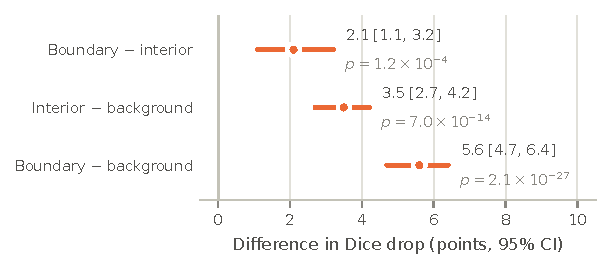
\includegraphics[width=\columnwidth]{figures/fig3_h2_pairwise.pdf}
  \caption{Paired differences in the drop in Dice between spot placements at SSIM~0.90 (points, threshold~0.5).
  Points are means over test images, bars 95\% bootstrap intervals; $p$-values from Wilcoxon signed-rank tests,
  Holm-corrected over the three comparisons.}
  \label{fig:h2}
\end{figure}

% Mechanism figure. Either a new figure next to Fig. 4 (change maps), or Fig. 4 itself if the maps are dropped.
\begin{figure}[t]
  \centering
  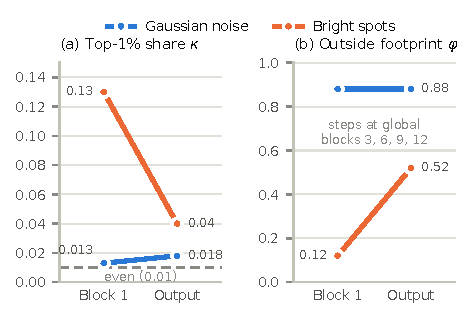
\includegraphics[width=\columnwidth]{figures/fig_mechanism_layer_spread.pdf}
  \caption{Spread of the encoder change at SSIM~0.90, after the first block and at the encoder output (means over
  20 test images). (a)~Share of the change carried by the 1\% most-changed tokens, $\kappa$ (dashed: even map).
  (b)~Share of the change outside the spots' footprint, $\varphi$; for spots it rises in steps at the global
  attention blocks 3, 6, 9 and 12. Lines join the two layers shown and do not trace the blocks between them.}
  \label{fig:layers}
\end{figure}
